This appendix provides a brief tutorial for the \julia\ package. We release this package on GitHub with the name \siplibjl. More detailed tutorial is provided in the GitHub repository.

\subsection{Prerequisites}
To use \siplibjl, you need to perform the following steps.
\begin{itemize}
	\item install the latest \julia\ release.
	\item install \julia\ packages: \texttt{Distributions.jl}, \texttt{JuMP.jl}, \texttt{StructJuMP.jl}, \texttt{PyPlot.jl}
	\item change working directory to ``\texttt{$\sim$/Siplib/src/}''
	\item run \julia\
	\item excute \texttt{include("Siplib.jl")}
	\item excute \texttt{using Siplib}
\end{itemize}
Then, you are all set to use the functions in \siplibjl.

\subsection{Generating instances: \texttt{JuMP.Model}-object and \smps\ files}
\jumpmodel-type object is an object that contains every information of an instance. Hence, almost every function in \siplibjl\ requires \jumpmodel-type object as one of its input arguments. \siplibjl\ provides two functions to construct the \jumpmodel-type object of an instance.
\begin{lstlisting}[frame=single,language=julia]
function getJuMPModel(problem::Symbol, param_arr::Any)::JuMP.Model
function generateSMPS(problem::Symbol, param_arr::Any, DIR_NAME::String="$(dirname(@__FILE__))/../instance")::JuMP.Model
\end{lstlisting}

The first function \texttt{getJuMPModel} takes \texttt{Symbol}-typed argument \texttt{problem} and associated parameter array \texttt{param\_arr}. Then, it constructs \jumpmodel-type object and return it. For example, the follwing command returns the \jumpmodel\ object of instance DCAP\_3\_4\_2\_100.
\begin{lstlisting}[frame=single,language=julia]
getJuMPModel(:DCAP, [3,4,2,100])
\end{lstlisting}
Keep in mind that the number of elements in \texttt{param\_arr} should match with the problem as in Table \ref{table:numparameter}, otherwise it prints a warning message.

\begin{table}[h]
	\centering
	\caption{\texttt{problem} arguments and corresponding parameter array}
	\label{table:numparameter}
	\resizebox{\textwidth}{!}{%
		\begin{tabular}{@{}ccc@{}}
			\toprule
			\texttt{problem}  & \texttt{param\_arr}     & Remark                                                                                                                                     \\ \midrule
			\texttt{:DCAP}               & \texttt{[R, T, N, $\mathcal{S}$]} & All parameters are integer.                                                                                                                \\
			\texttt{:MPTSPs}             & \texttt{[D, N, $\mathcal{S}$]}    & String $\texttt{D}\in \{\mathrm{``D0"}, \mathrm{``D1"}, \mathrm{``D2"}, \mathrm{``D3"}\}$                                                              \\
			\texttt{:SIZES}              & \texttt{[$\mathcal{S}$]}          & Integer $\mathcal{S}\ge 20$.                                                                                   \\
			\texttt{:SMKP}               & \texttt{[I, $\mathcal{S}$]}       & All parameters are integer.                                                                                                                \\
			\texttt{:SSLP}               & \texttt{[I, J, $\mathcal{S}$]}    & All parameters are integer.                                                                                                                \\
			\texttt{:SUC}                & \texttt{[D, $\mathcal{S}$]}       & \multicolumn{1}{l}{String $\texttt{D}\in \{\mathrm{``FallWD"}, \mathrm{``FallWE"}, \mathrm{``WinterWD"}, \mathrm{``WinterWE"}, $}                                             \\
			\multicolumn{1}{l}{}         & \multicolumn{1}{l}{}            & \multicolumn{1}{r}{$\mathrm{``SpringWD"}, \mathrm{``SpringWE"}, \mathrm{``SummerWD"}, \mathrm{``SummerWE"} \}$} \\ \bottomrule
		\end{tabular}
	}
\end{table}

The second function \texttt{generateSMPS} generates \smps\ files as well as returns \jumpmodel\ object by taking one more argument \texttt{DIR\_NAME} to indicate a directory where the files are stored. The \smps\ files are stored in the default folder ``\texttt{$\sim$/Siplib/instance/}'' unless the argument \texttt{DIR\_NAME} is specified. The file name is automatically generated using the arguments, e.g., \texttt{generateSMPS(:DCAP, [3, 4, 2, 100])} generates three files.
\begin{itemize}
	\item DCAP\_3\_4\_2\_100.cor
	\item DCAP\_3\_4\_2\_100.tim
	\item DCAP\_3\_4\_2\_100.sto
\end{itemize}
Sometimes one might want to generate \smps\ files using pre-declared \texttt{JuMP.Model} object. The function \texttt{writeSMPS} is defined to do such task.
\begin{lstlisting}[frame=single,language=julia]
function writeSMPS(model::JuMP.Model, INSTANCE::String="instance", DIR_NAME::String="$(dirname(@__FILE__))/../instance")
\end{lstlisting}
The function above takes \jumpmodel\ object as input argument and stores \smps\ files into \texttt{DIR\_NAME} folder with file name \texttt{INSTANCE}. The \texttt{String}-type arguments \texttt{INSTANCE} and \texttt{DIR\_NAME} can be omitted since they have default values ``\texttt{instance}" and ``\texttt{$\sim$/Siplib/instance/}."

We also define a conventional function to return the instance name in \texttt{String}-type.
\begin{lstlisting}[frame=single,language=julia]
function getInstanceName(problem::Symbol, param_arr::Any)::String
\end{lstlisting}

\subsection{Pre-analyzing instances: size, sparsity, plot}
\siplibjl\ provides pre-analysis functions for instances. By ``size'', we mean the number of components (continuous, binary, integer, constraint) in an instance. As we discussed in Section \ref{sec:sparsity}, sparsity is analyzed in block-wisely. The size and sparsity information is stored in the object of the following types: \texttt{Size} and \texttt{Sparsity}.

\siplibjl\ also provides functions to plot sparsity pattern in the coefficient matrix. The plots can be drawn in four ways. 
\begin{itemize}
	\item Coefficient matrix of extensive form
	\item First stage-only block (block A)
	\item Second stage-only block (block W)
	\item Technology block (block T)
\end{itemize}

%\kk{This section looks more or less a manual; but, should provide more than that. For example, the section should contain the answers to the questions: Why do we care about this? What kind of information do we want to provide? Does it provide any information for testing algorithms? The manual-like information would better go to the package website (not research paper).}
%\yoc{The answers to the questions are discussed in Section 3: the reasons why variable types, number of components (size), sparsity are important.}

%\noindent\begin{minipage}{.45\textwidth}
%\begin{lstlisting}[frame=single,language=julia]
%type Size
%	InstanceName::String
%	nCont1::Int
%	nBin1::Int
%	nInt1::Int
%	nCont2::Int
%	nBin2::Int
%	nInt2::Int
%	nCont::Int
%	nBin::Int
%	nInt::Int
%	nRow::Int
%	nCol::Int
%	nNz::Int
%	Size() = new()
%end
%\end{lstlisting}
%\end{minipage}\hfill
%\begin{minipage}{.45\textwidth}
%\begin{lstlisting}[frame=single,language=julia]
%type Sparsity
%	InstanceName::String
%	nRow1::Int
%	nCol1::Int
%	nNz1::Int
%	sparsity1::Float64
%	nRow2::Int
%	nCol2::Int
%	nNz2::Int
%	sparsity2::Float64
%	nRowC::Int
%	nColC::Int
%	nNzC::Int
%	sparsityC::Float64
%	nRow::Int
%	nCol::Int
%	nNz::Int
%	sparsity::Float64
%	Sparsity() = new()
%end
%\end{lstlisting}
%\end{minipage}

\subsubsection{Get size information}
To get the size information of an instance, excute the following function.
\begin{lstlisting}[frame=single,language=julia]
function getSize(model::JuMP.Model, InstanceName::String="")::Size
\end{lstlisting}
The function \texttt{getSize} takes \jumpmodel\ as an input argument and returns \texttt{Size}-type object defined as follows.
\begin{lstlisting}[frame=single,language=julia]
type Size
	InstanceName::String    # instance name
	nCont1::Int             # number of continuous variables in 1st stage
	nBin1::Int              # number of binary variables in 1st stage
	nInt1::Int              # number of integer variables in 1st stage
	nCont2::Int             # number of continuous variables in 2nd stage    
	nBin2::Int              # number of binary variables in 2nd stage
	nInt2::Int              # number of integer variables in 2nd stage    
	nCont::Int              # number of continuous variables in total      
	nBin::Int               # number of binary variables in total      
	nInt::Int               # number of integer variables in total      
	nRow::Int               # number of rows in coefficient matrix in extensive form
	nCol::Int               # number of columns in coefficient matrix in extensive form
	nNz::Int                # number of nonzero values in coefficient matrix in extensive form
	Size() = new()
end
\end{lstlisting}

\subsubsection{Get sparsity information}
To get the sparsity information of an instance, excute the following function.
\begin{lstlisting}[frame=single,language=julia]
function getSparsity(model::JuMP.Model, InstanceName::String="")::Sparsity
\end{lstlisting}
The function \texttt{getSparsity} takes \jumpmodel\ as an input argument and returns \texttt{Sparsity}-type object.
\begin{lstlisting}[frame=single,language=julia]
type Sparsity
	InstanceName::String    # instance name
	nRow1::Int              # number of rows in 1st stage-only block (block A)
	nCol1::Int              # number of columns in 1st stage-only block (block A)
	nNz1::Int               # number of nonzero values in 1st stage-only block (block A)
	sparsity1::Float64      # sparsity ([0,1] scale) of 1st stage-only block (block A)
	nRow2::Int              # number of rows in 2nd stage-only block (block W)
	nCol2::Int              # number of columns in 2nd stage-only block (block W)
	nNz2::Int               # number of nonzero values in 2nd stage-only block (block W)
	sparsity2::Float64      # sparsity ([0,1] scale) of 2nd stage-only block (block W)
	nRowC::Int              # number of rows in technology block (block T)
	nColC::Int              # number of columns in technology block (block T)
	nNzC::Int               # number of nonzero values in technology block (block T)  
	sparsityC::Float64      # sparsity ([0,1] scale) of technology block (block T)
	nRow::Int               # number of rows in total
	nCol::Int               # number of columns in total
	nNz::Int                # number of nonzero values in total
	sparsity::Float64       # sparsity ([0,1] scale) in total
	Sparsity() = new()
end
\end{lstlisting}
\subsubsection{Plot sparsity patterns}
To plot the sparsity patterns of coefficient matrices, we provide the following functions.
\begin{lstlisting}[frame=single,language=julia]
function plotConstrMatrix(model::JuMP.Model, INSTANCE::String="instance", DIR_NAME::String="$(dirname(@__FILE__))/../plot")

function plotFirstStageBlock(model::JuMP.Model, INSTANCE::String="instance_block_A", DIR_NAME::String="$(dirname(@__FILE__))/../plot")

function plotSecondStageBlock(model::JuMP.Model, INSTANCE::String="instance_block_W", DIR_NAME::String="$(dirname(@__FILE__))/../plot")

function plotComplicatingBlock(model::JuMP.Model, INSTANCE::String="instance_block_T", DIR_NAME::String="$(dirname(@__FILE__))/../plot")

function plotAllBlocks(model::JuMP.Model, INSTANCE::String="instance", DIR_NAME::String="$(dirname(@__FILE__))/../plot")

function plotAll(model::JuMP.Model, INSTANCE::String="instance", DIR_NAME::String="$(dirname(@__FILE__))/../plot")
\end{lstlisting}
The function \texttt{plotConstrMatrix} takes \jumpmodel-type object and plots the constraint matrix of extensive form. For example, the following command lines plot Fig. \ref{fig:plotall_b}.
\begin{lstlisting}[frame=single,language=julia]
param_arr = [2,2,2,2]	                        # declare parameters
problem = :DCAP	                                # declare problem
INSTANCE = getInstanceName(problem, param_arr)	# save instance name
model = getJuMPModel(problem, param_arr)	    # construct JuMP.Model object
plotConstrMatrix(model, INSTANCE)               # plot extensive form constraint matrix   
\end{lstlisting}

The functions \texttt{plotFirstStageBlock}, \texttt{plotSecondStageBlock}, and \texttt{plotComplicatingBlock} take \jumpmodel-type object and plots each block. For example, the following command lines plot Fig. \ref{fig:plotall_a}, \ref{fig:plotall_c}, and \ref{fig:plotall_d}.
\begin{lstlisting}[frame=single,language=julia]
param_arr = [2,2,2,2]	                        # declare parameters
problem = :DCAP	                                # declare problem
INSTANCE = getInstanceName(problem, param_arr)	# save instance name
model = getJuMPModel(problem, param_arr)	    # construct JuMP.Model object
plotFirstStageBlock(model, INSTANCE)               # plot 1st stage block
plotSecondStageBlock(model, INSTANCE)               # plot 2nd stage block
plotComplicatingBlock(model, INSTANCE)               # plot technology block
\end{lstlisting}

One might want to draw all the plots at once. The following two functions are defined to do that.
\begin{lstlisting}[frame=single,language=julia]
plotAllBlocks(model, INSTANCE)               # plot all blocks A,W,T
plotAll(model, INSTANCE)               # plot all the plots above
\end{lstlisting}
\begin{figure}[H]
	\centering
	\subfloat[][DCAP\_2\_2\_2\_2\_block\_A.pdf]
	{
		\centering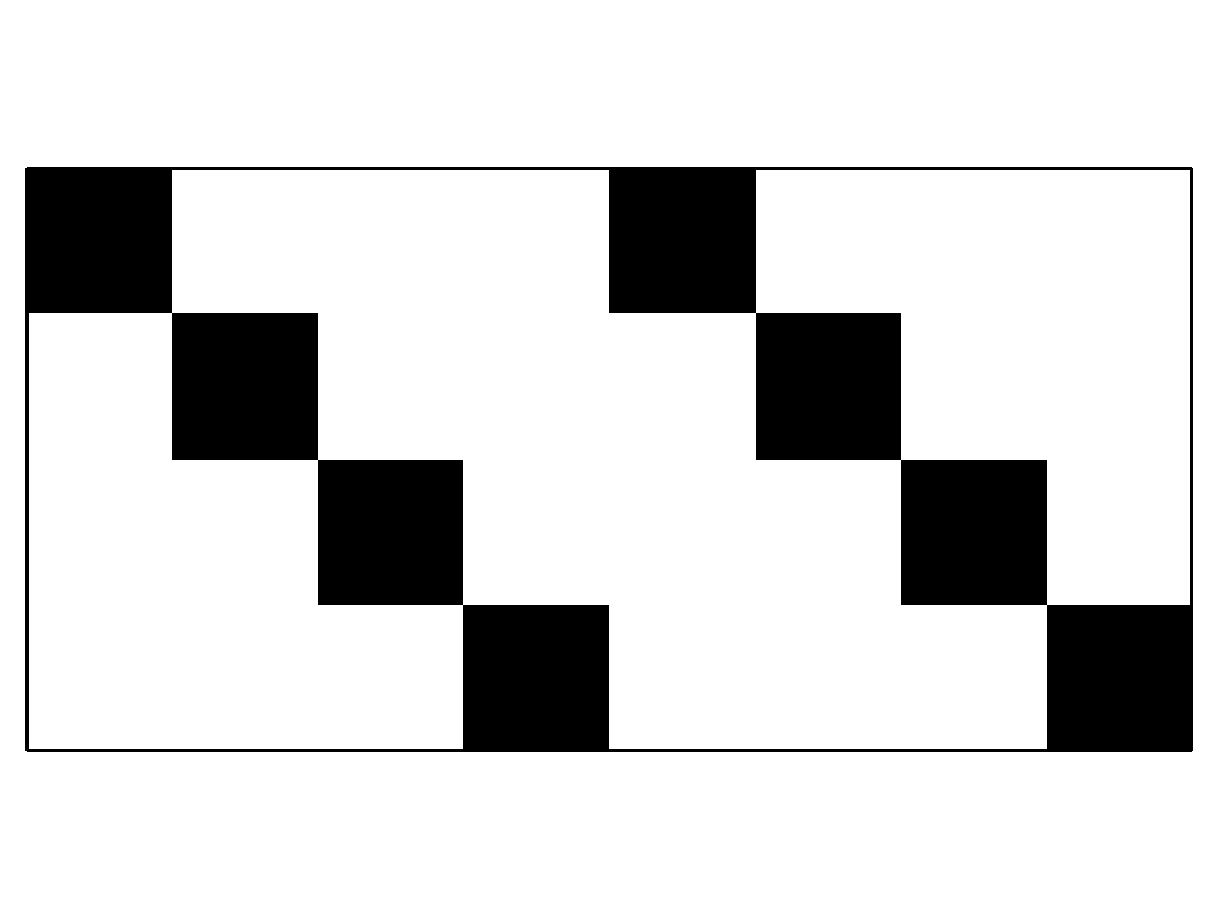
\includegraphics[width=0.45\linewidth]{DCAP_2_2_2_2_block_A}
		\label{fig:plotall_a}
	}
	~
	\subfloat[][DCAP\_2\_2\_2\_2.pdf]
	{
		\centering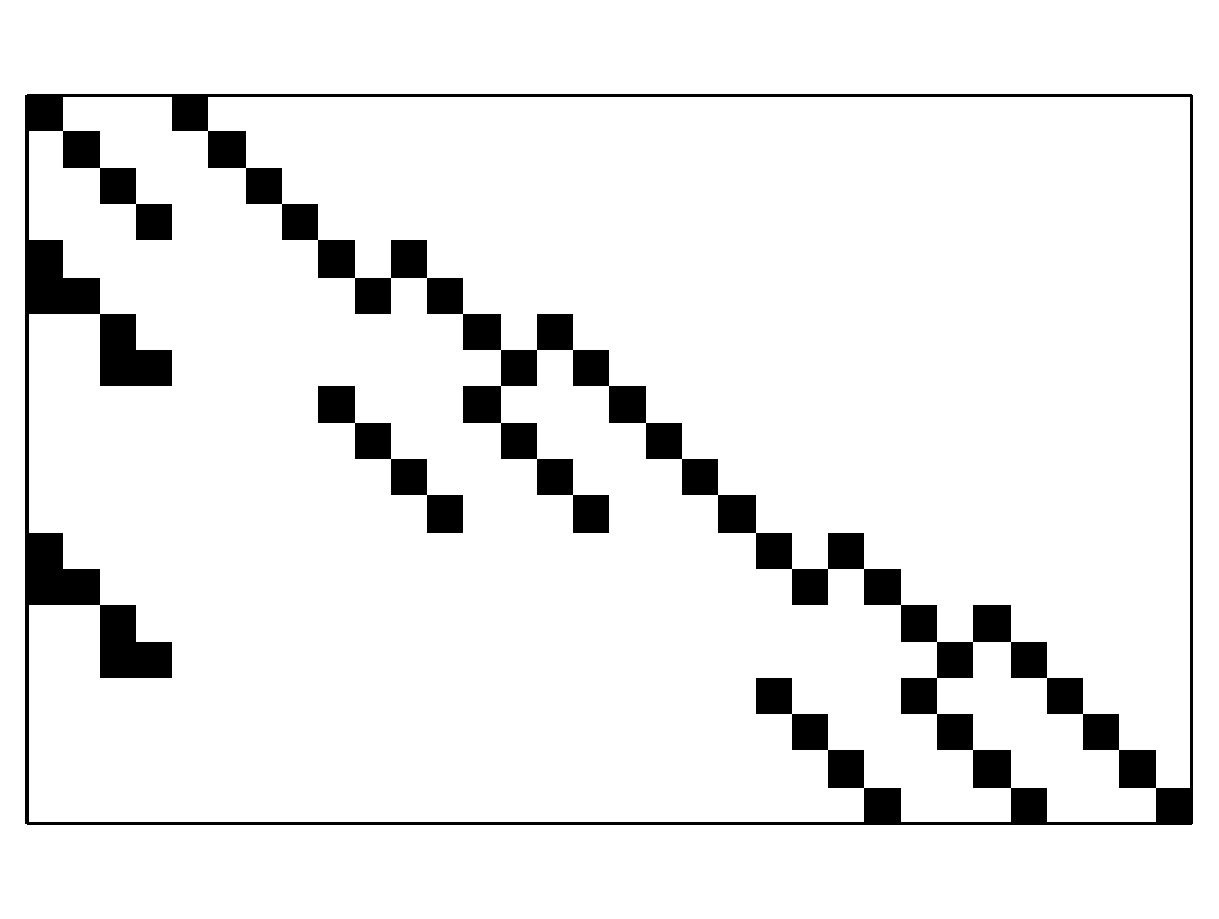
\includegraphics[width=0.45\linewidth]{DCAP_2_2_2_2}
		\label{fig:plotall_b}
	}
	
	\subfloat[][DCAP\_2\_2\_2\_2\_block\_T.pdf]
	{
		\centering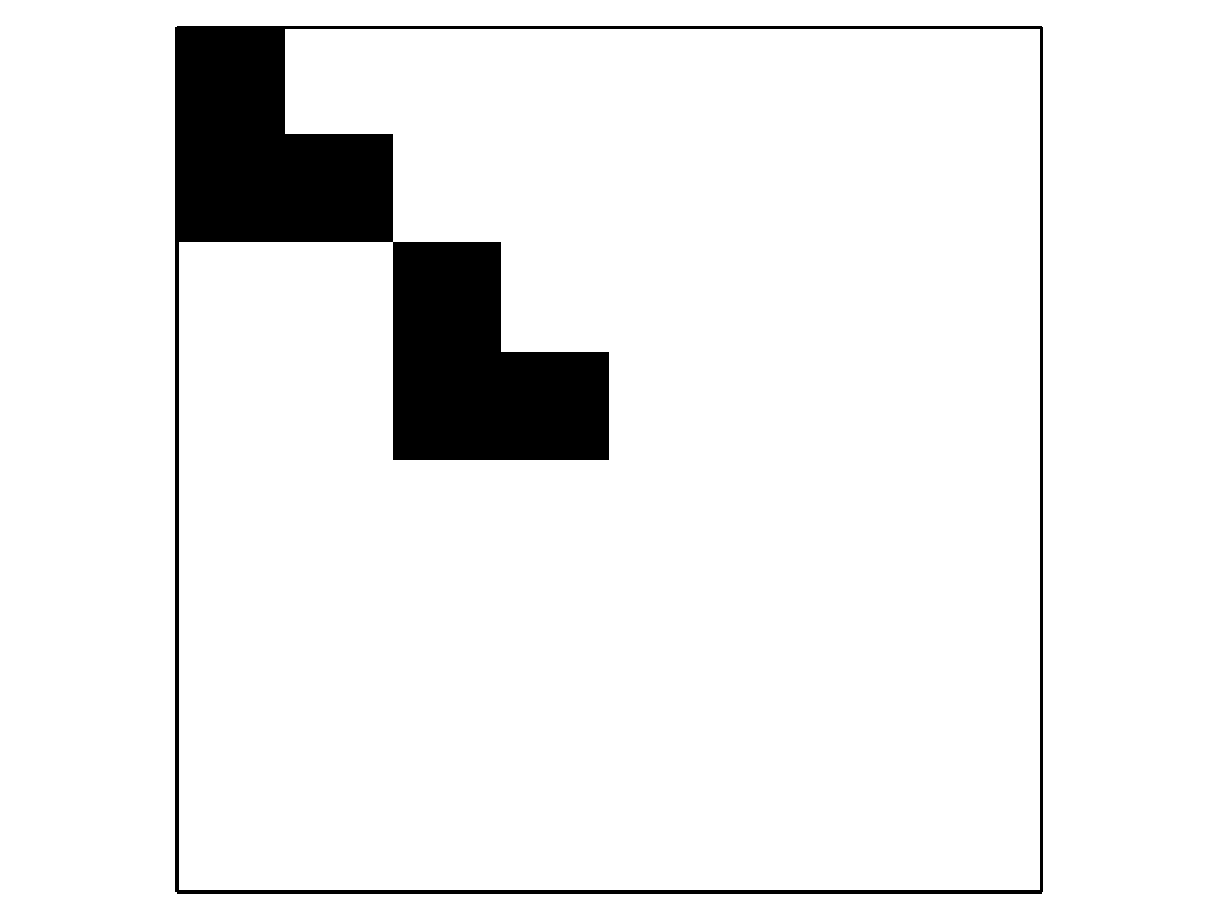
\includegraphics[width=0.45\linewidth]{DCAP_2_2_2_2_block_T}
		\label{fig:plotall_c}
	}
	~
	\subfloat[][DCAP\_2\_2\_2\_2\_block\_W.pdf]
	{
		\centering
\includegraphics[width=0.45\linewidth]{DCAP_2_2_2_2_block_W}
		\label{fig:plotall_d}
	}

	\caption{Plots drawn by executing function \texttt{plotAll}}
%	\begin{minipage}
%	\end{minipage}
	\label{fig:plotall}
\end{figure}
By executing \texttt{plotAll}, one can obtain all the plots in Fig. \ref{fig:plotall}.

%\kk{This subsection can probably be removed from the paper and should go to a manual or a repository. Otherwise, please describe why/how this can be used for research.}
%\yoc{I move this to appendix. We can remove this.}

%
%\subsection{Solving instances: interfacing with \texttt{DSP} solver}
%\subsubsection{Extensive form: Invoking standard MIP solver}
%
%\subsubsection{Dual decomposition}
%
%\subsubsection{Benders decomposition}